\chapter{Introducción}
\label{chap:introduction}

%%% FILL IN YOUR LINKS BELOW! %%%

\begin{center}
    \begin{minipage}{.85\linewidth}
    \begin{linkbox}
        \textbf{Github link:} \url{https://github.com/jblanp03/dps}\\
        % \textbf{Screencast link:} \url{...}
        \textbf{DPS en Agora:}
        \href{https://agora.unileon.es/course/view.php?id=3060}{agora.unileon.es} \\
       
    \end{linkbox}
    \end{minipage}
\end{center}




\section{Introducción}

El presente documento muestra la aplicación de las 5 fases del libro Secure Coding Principles and  Practices \cite{wikimedia:2017} a un proyecto consistente en el desarrollo de un asistente virtual de texto. Este documento tiene como objetivo poder evaluar la seguridad del proyecto presentado a partir de unos principios que se centran en evaluar distintos aspectos del software, como la calidad del sistema y el desarrollo seguro. Las 5 fases que se utilizan para dicha evaluación son:

\begin{itemize}
    \item Arquitectura
    \item Diseño
    \item Implementación
    \item Operaciones
    \item Automatización y test
\end{itemize}




\section{Descripción del proyecto}

El proyecto a evaluar es un desarrollo de asistente virtual, chatbot de flujo pregunta-respuesta guiado, desplegado en un entorno web que pretende mantener una conversación guiada con el usuario final, alumnos de un curso, con el objetivo de obtener un feedback más detallado acerca tanto del desempeño del curso como de los agentes participantes (instructores, ponencias, etc.), instalaciones y materiales, lecturas, etc. En una fase ajena al sistema desarrollado, los alumnos completan un cuestionario proporcionando un feedback sobre el curso. En funcion de las respuestas se generan tres tipos de usuarios finales:



\begin{itemize}
    \item Usuario nivel 0: Usuarios con nivel de satisfacción es 100\%.
    \item Usuario nivel 1: Usuarios con nivel de satisfacción se encuentra entre 75-99\%
    \item Usuario nivel 2: Usuarios con nivel de satisfacción es superior a 50\% e inferior a 75\%
    \item Usuario nivel 3: Son usuarios cuyo nivel de satisfacción es inferior al 50\%.
\end{itemize}

El uso de distintos perfiles de usuarios es para elaborar un flujo de pregunta-respuesta por parte del chatbot distinto, aunque de cara a la activación y uso del chatbot, todos los usuarios lo realizan de la misma manera. Los alumnos que estén registrados en la base de datos del sistema, es decir, aquellos que el centro haya registrado su cuestionario, se les proporcionará un código de forma manual con el que podrán activar este chatbot instalado en un entorno web. Si los usuarios acceden al chatbot previo a tener registrado sus respuestas del cuestionario, el chatbot no les permitirá activar el flujo.


\begin{figure}[h]
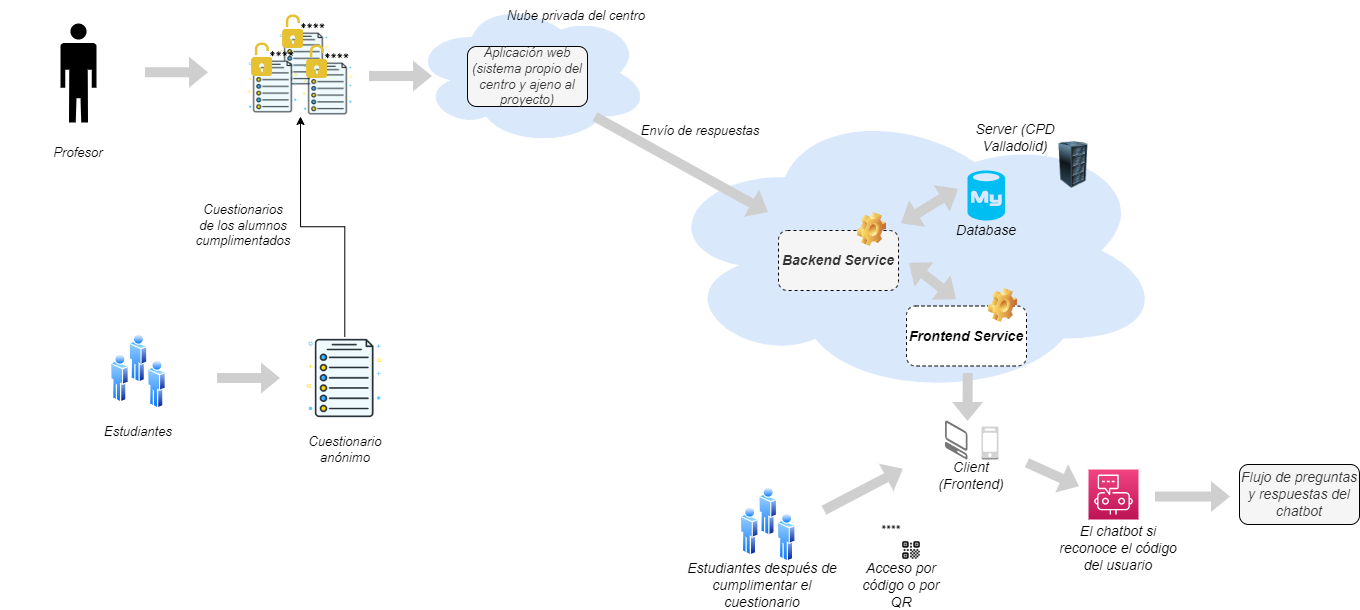
\includegraphics[width=\textwidth]{figures/EsquemaGeneral.png}
\caption{Esquema general}
\label{fig:esquema}
\end{figure}

Procedimiento:

\begin{enumerate}
    \item El profesor de la formación imprime un cuestionario de valoración que los alumnos deben cumplimentar en el aula. A cada cuestionario les proporciona un código de 6 dígitos y un código QR. El profesor se queda con una copia para asignar las respuestas posteriormente dentro de un sistema propio.
    \item Con el cuestinario cumplimentado, el profesor introduce las respuestas y el sistema obtiene el grado de satisfacción de cada alumno. Se almacena su grado de satisfacción relacionado con el código (anónimo).
    \item El sistema del asistente virtual interpreta dicho código y su grado de satisfacción y le asigna un tipo de usuario para el flujograma del proceso lógico.
    \item El usuario accede al servicio del asistente para interactuar y el asistente detecta el código y su tipo de usuario.
    \item El asistente entabla conversación con el usuario en función del flujograma de preguntas y respuestas.
    \item Finaliza el flujograma y se finaliza el proceso.
\end{enumerate}